\documentclass{article}
\usepackage{graphicx}% Required for inserting images
\usepackage{lindrew}
\usepackage{pdfpages}
\usepackage{amsmath}
\usepackage{algorithm}
\usepackage{enumitem}
\usepackage{algpseudocode}
\usepackage{matlab-prettifier}
\usepackage{pythonhighlight}
\title{CS 156a Final}
\author{Amitesh Pandey}
\date{December 2024}

\begin{document}
\maketitle
\subsection*{Problem 1}
Let's take a point $(x, y)$ of dimension $d = 2$ and first apply a polynomial transform of dimension $Q = 2$. 
\begin{equation*}
    (x, y) = (x, y, xy, x^2, y^2) = (x^1 y^0, x^0 y^1, x^1 y^1, x^2 y^0, x^0 y^2)
\end{equation*}
We can think of this as a counting problem where we must count all possible permutations of the exponents of $x$ and $y$ such that their sum does not exceed $Q$. For $Q = 10$, note that none of the two exponents can exceed 10 since it isn't permissible to have the other exponent negative. Also observe that if we pick $\alpha$ as the exponent for $x$, then we $11 - \alpha$ choices for the exponent of $y$, say $\beta$. Now $\alpha$ itself can range from $0$ to $10$. So the dimension $d'$
\begin{equation*}
    d' = \sum_{\alpha = 0}^{10} (11 - \alpha ) = 66
\end{equation*}
We will have a transform of the form
\begin{equation*}
    (x, y) \to (1, x, x^2, x^3, \dots, x^5 y^5, \dots, y^{10})
\end{equation*}
Notice that this does include the constant coordinate $1$ produced by the exponent arrangement $x^0 y^0$, ignoring this, we get a total dimension of 65. So the correct option is $\textbf{[e]}$. 
\subsection*{Problem 2}
For this problem,
\begin{enumerate}[label=\textbf{[\alph*]}]
    \item If $\mathcal{H}$ has only one hypothesis, say $h$, then for all $\mathcal{D}_{1}, \mathcal{D}_{2}, \dots, \mathcal{D}_{n}$, we have $g^{(\mathcal{D})} = h$. This implies that $\Bar{g} = \frac{1}{n}\cdot (h + h + \dots + h) = h$. But we know that $h \in \mathcal{H}$. 
    \item Say for $\mathcal{D}_{k}$, the received hypothesis is $g^{(\mathcal{D}_k)} = a_{k}$. Then $\Bar{g} = \frac{1}{n}\left(a_{1} + \dots + a_{n}\right)$. This is a real value, so $\Bar{g} \in \mathcal{H}$. 
    \item Say for $\mathcal{D}_{k}$, the received hypothesis is $g^{(\mathcal{D}_k)} = a_{k}x + b_{k}$. Then $\Bar{g} = \frac{1}{n}\left(a_{1}x + b_{1} + \dots + a_{n}x + b_{n}\right)$. On refactorising, we get $\Bar{g} = \frac{1}{n}\left(a_{1} + \dots + a_{n}\right)x + \frac{1}{n}\left(b_{1} + \dots + b_{n}\right)$. Both are real values, so we have $\Bar{g} \in \mathcal{H}$. 
    \item Say for $\mathcal{D}_{k}$, the received hypothesis $g^{(\mathcal{D}_{k})} = \frac{1}{1 + e^{-(a_{k} + b_{k}x)}}$. Then
    \begin{equation*}
        \Bar{g} = \frac{k + e^{-(a_{1} + b_{1}x) } + e^{-(a_{2} + b_2x)} + \dots + e^{-(a_{n} + b_n x)}}{(1 + e^{-(a_{1} + b_{1}x)})(1 + e^{-(a_{2} + b_{2}x)})\dots (1 + e^{-(a_{n} + b_{n}x)})}
    \end{equation*}
\end{enumerate}
Clearly $\Bar{g} \notin \mathcal{H}$, so the correct option is $\textbf{[d]}$. 
\newpage
\subsection*{Problem 3}
Suppose there are two hypotheses $h, h'$. By definition, $h'$ overfits relative to $h$ if it achieves a lower in-sample-error, say $E_{\text{in}}'$, but a higher out-sample-error, say $E_{\text{out}}'$ than $h$. Assume $h$ achieves in-sample-error $E_{\text{in}}$ and out-sample-error $E_{\text{out}}$. Naturally, $E_{\text{in}} \neq E_{\text{in}}'$ and $E_{\text{out}} \neq E_{\text{out}}'$. It follows then that $E_{\text{out}}' - E_{\text{in}}' \neq E_{\text{out}} - E_{\text{in}}$. More specifically, $E_{\text{out}}' - E_{\text{in}}' > E_{\text{out}} - E_{\text{in}}$. This inequality makes it clear that overfitting detection requires some sort of a \emph{baseline} $E_{\text{out}} - E_{\text{in}}$ level to which a hypothesis' results need to be compared. This means that overfitting cannot be determined with only one hypothesis. This eliminates options $\textbf{[a]}, \textbf{[b]}, \textbf{[c]}, \textbf{[e]}$. The main problem with comparing only $E_{\text{out}} - E_{\text{in}}$ values is that generally, a hypothesis overfits relative to another not only if the difference in its out-sample and in-sample errors are large, but also that this large difference is necessarily produced by a large $E_{\text{out}}$ and a relatively small $E_{\text{in}}$, or that the hypothesis has \emph{overfit} the data. This detail is lost in comparing only the difference value. So the correct option is $\textbf{[d]}$.
\subsection*{Problem 4}
\emph{Deterministic noise} refers to the component of noise borne out of a foundational difference in the complexity of the data and the capacity of the hypothesis set. \emph{Stochastic noise} refers to more \emph{random} noise that's a result of inaccurate measurements, random processes intercepting the data-generation method etc. With this in mind
\begin{enumerate}[label = \textbf{[\alph*]}]
    \item Stochastic and deterministic noise do not contradict each other. The processes that they originate from can coexist. So this statement is false.
    \item Since deterministic noise is in some sense a reflection of the hypothesis sets' incapacity, we can conclude that it does depend on the hypothesis sets. So this statement is false.
    \item Since deterministic noise is in some sense a reflection of the target function's complexity, we can conclude that it does depend on the target function. So this statement is false.
    \item Since stochastic noise deals more with randomness in the ``input" side of the learning diagram, I would imagine it is not effected by our choice of hypotheses. So this is true.
    \item As stated previously, stochastic noise is a measure of the randomness in the distribution of $\mathcal{X}$ and the randomness of the target function. So this statement is false.
\end{enumerate}
In conclusion, option $\textbf{[d]}$ is correct.
\subsection*{Problem 5}
Recall that the unconstrained solution to the regularization problem is $\mathbf{w}_{\text{lin}}$. Now we're given in the question that this vector satisfies the Tikhonov constraint. Then, this is also the constrained solution. So $\mathbf{w}_{\text{reg}} = \mathbf{w}_{\text{lin}}$, so $\textbf{[a]}$.
\subsection*{Problem 6}
Soft order constraints that regularise polynomials can be used to regularise the hypothesis, in this case, they are directly associated with the augmented error. So $\textbf{[b]}$ is the correct option.
\newpage
\subsection*{Problem 7}
Using the code in the appendix, with only the bias $(x_{1}, x_{2}) \to (1, x_1, x_2)$, we get that the ``8 versus all" classifier has the smallest $E_{\text{in}}$ with $E_{\text{in}} \approx 0.74$. The correct option is $\textbf{[d]}$.
\subsection*{Problem 8}
Using the code in the appendix, with the transform $(x_1, x_2) \to (x_1, x_2, x_1 x_2, x_{1}^{2}, x_{2}^2)$, we get that the ``1 versus all" classifier has the smallest $E_{\text{out}}$ with $E_{\text{out}} \approx 0.02$, so the correct option is $\textbf{[b]}$.
\subsection*{Problem 9}
Using the code in the appendix, we get that only $\textbf{[e]}$ is correct, $E_{\text{out}}$ is lower using the transform than not but the improvement is less than 1\%. 
\subsection*{Problem 10}
Using the code in the appendix, we get that only $\textbf{[a]}$ is correct.
\subsection*{Problem 11}
Using the code in the appendix, we get the plot of transformed points as:
\begin{figure}[htp]
    \centering
    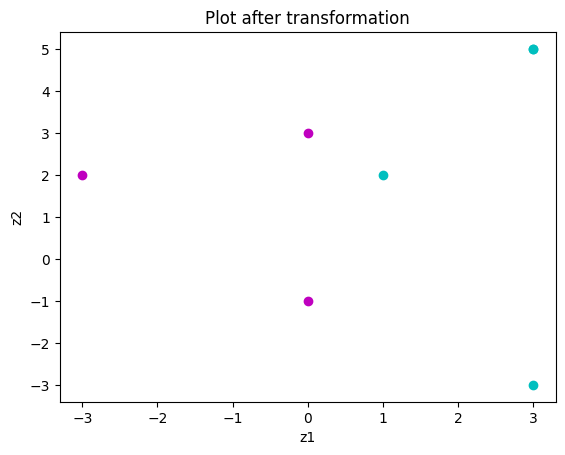
\includegraphics[width=2in]{plotfinal.png}
    \label{fig:galaxy}
\end{figure}
\\\\This means that the margin maximizing plane must cut at $z_1 = 0.5$. Since $z_2$ does not change the label of the point, $w_2 = 0$. If the plane is given by $\langle w_1, w_2 \rangle^{T}z + b = 0$, on putting $z_1 = 0.5$ and $z_2 = 0$, and $w_2 = 0$, we get that $b = -0.5$. Note that we could just as easily pick any other point on the line of intersection but this was the most convenient. So the final solution is $1, 0, -0.5$ or option $\textbf{[c]}$.
\subsection*{Problem 12}
Using the code in the appendix, the optimal occurs when $C \geq 10$, and the number of support vectors in this case is 5, so range 4-5, or $\textbf{[c]}$ is correct.
\subsection*{Problem 13}
From code in the appendix, the dataset was inseparable by the kernel RBF $0.0\%$ of the times, so $\textbf{[a]}$ is correct.
\subsection*{Problem 14}
From the code in the appendix, we get that RBF kernel beats RBF regular 93\% of the times, in terms of $E_{\text{out}}$. This means that $\textbf{[e]}$ is the correct option.
\subsection*{Problem 15}
From the code in the appendix, we get that for $K = 12$, RBF kernel beats RBF regular 82\% of the times, which is between 60\% and 90\% so $\textbf{[d]}$ is the correct option.
\subsection*{Problem 16}
From the code in the appendix, we get that $E_{\text{in}}$ goes down as $K$ (\verb|num_clusters|) goes up 83\% of the times as well as $E_{\text{out}}$ goes down as $K$ goes up 76\% of the times. Since it's most common for both to go down, $\textbf{[d]}$ is correct.
\subsection*{Problem 17}
From the code in the appendix, we get that $E_{\text{in}}$ goes up as $\gamma$ (\verb|num_clusters|) goes up 52\% of the times as well as $E_{\text{out}}$ goes up as $\gamma$ goes up 58\% of the times. Since it's most common for both to go up, $\textbf{[c]}$ is correct.
\subsection*{Problem 18}
From the code in the appendix, we get that exactly $0.0\%$ of the times is $E_{\text{in}} = 0$ achieved, so $\textbf{[a]}$ is correct.
\subsection*{Problem 19}
Given a single person $\mathcal{P}$ that had a heart attack, we know that $f \neq 0$. However we are not guaranteed that $f = 1$ either. This eliminates $\textbf{[a]}$ and $\textbf{[d]}$. This also implies that, $P(f=0 \mid \mathcal{P})=0$ and $P(0<f\leq 1 \mid \mathcal{P})\neq 0$. We can now determine whether $P(h=f \mid \mathcal{D})$ grows linearly or nonlinearly over $[0,1]$. From Bayes

$$
P(h=f \mid \mathcal{D})=\frac{P(\mathcal{D} \mid h=f) P(h=f)}{P(\mathcal{D})} \propto P(\mathcal{D} \mid h=f) P(h=f) \propto f P(h=f)
$$
We can draw the final conclusion because it is obvious that for a person, the probability that they have a heart attack \emph{given} that $h = f$ is $f$ itself. This means that it is a linear relation, so $\textbf{[b]}$ is correct.
\subsection*{Problem 20}
\begin{enumerate}[label=\textbf{[\alph*]}]
    \item If $g_1$ is much closer to the actual target than $g_2$ then the average becomes more erroneous because of $g_2$-introduced error, so this is false.
    \item If If $g_1$ is much closer to the actual target than $g_2$ then the average hypothesis becomes more erroneous because of $g_2$-introduced error, so the average error in this case will be higher than $E_{\text{out}}(g_1)$.
    \item Could be, because of some mean squared stuff.
    \item This option is essentially the same as $\textbf{[b]}$, which we eliminated.
\end{enumerate}
So finally, the answer is either option $\textbf{[c]}$ or $\textbf{[e]}$.
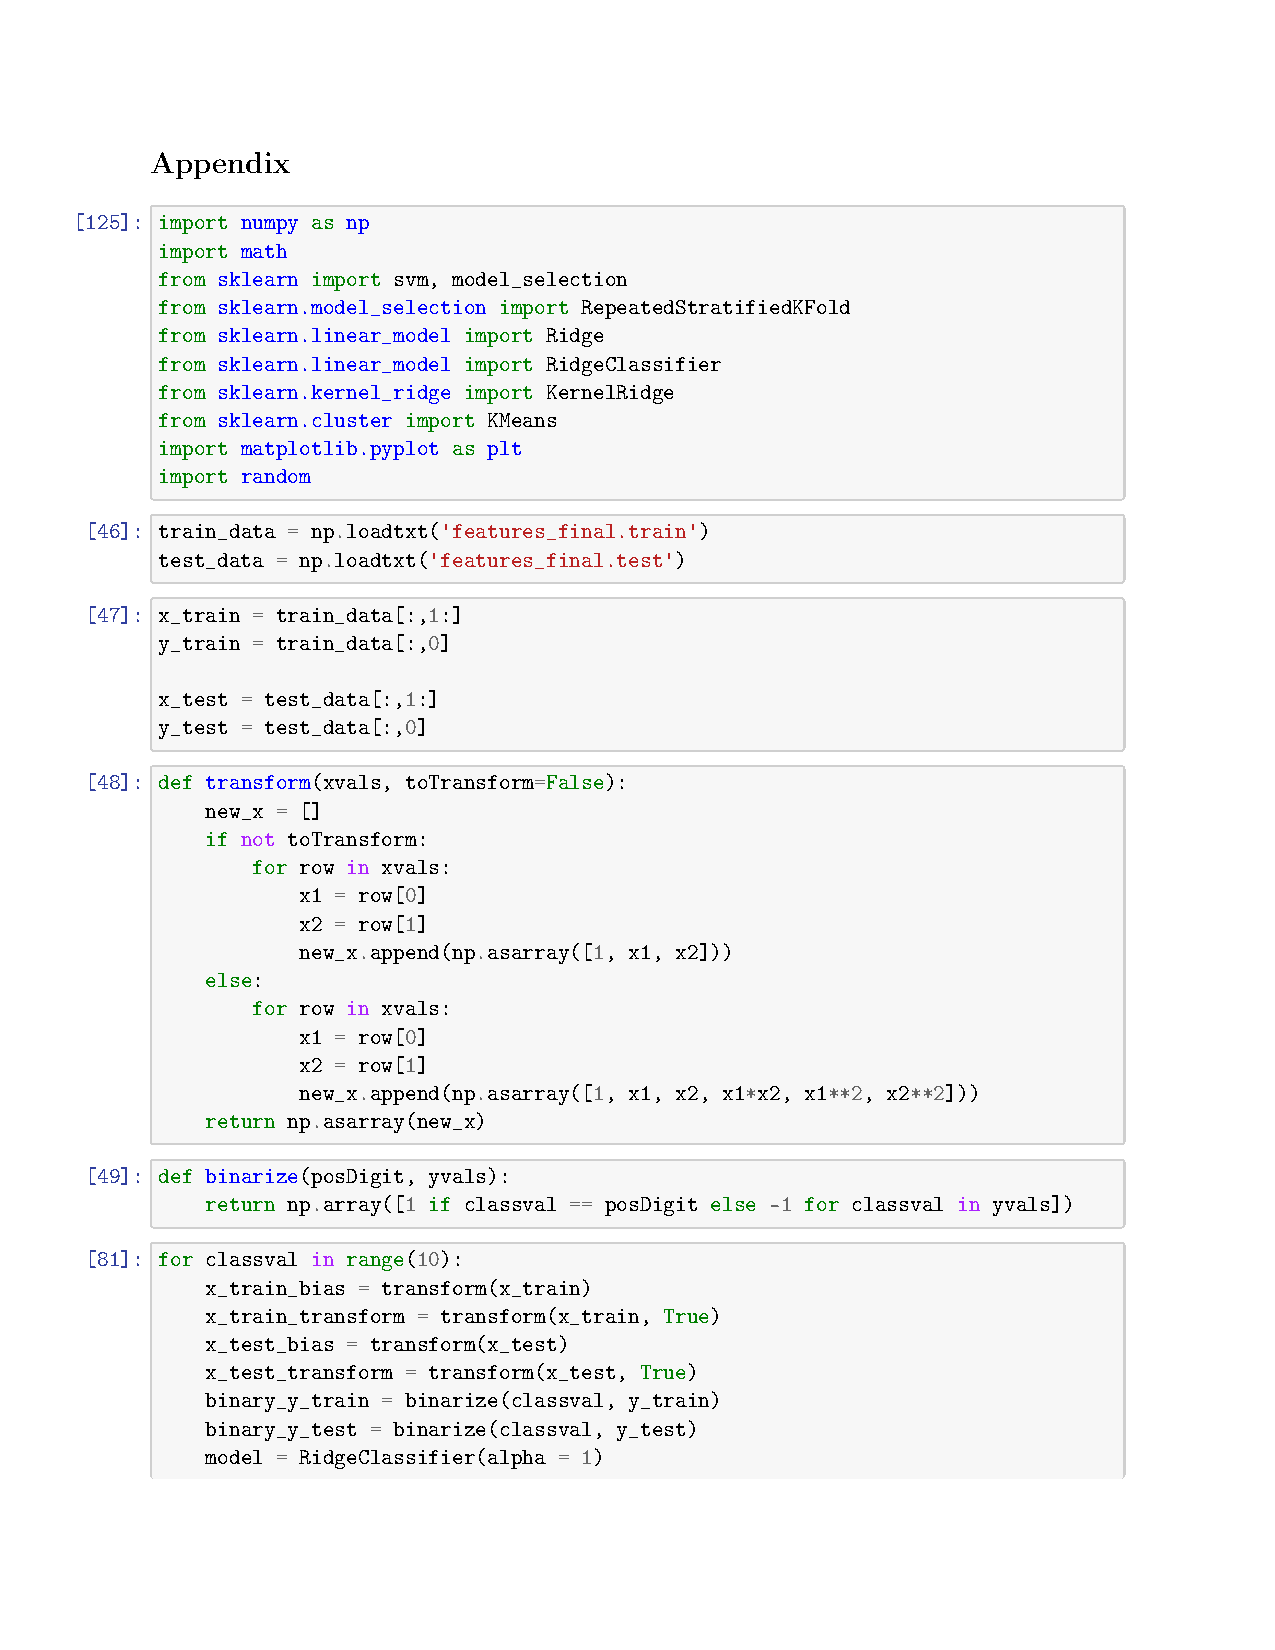
\includepdf[pages=-]{Code_for_Final.pdf}
\end{document}
